\documentclass{beamer}
\usetheme{Warsaw}

\definecolor{azure}{rgb}{0.0, 0.5, 1.0}
\definecolor{awesome}{rgb}{1.0, 0.13, 0.32}
\definecolor{darktangerine}{rgb}{1.0, 0.66, 0.07}
\definecolor{kellygreen}{rgb}{0.3, 0.73, 0.09}
\definecolor{lightseagreen}{rgb}{0.13, 0.7, 0.67}
\definecolor{cadmiumgreen}{rgb}{0.0, 0.42, 0.24}

\setbeamercolor{structure}{fg=cadmiumgreen!90!black}
\setbeamercovered{transparent}

\usepackage[english]{babel} 
\usepackage{algorithm,algpseudocode}
\usepackage{setspace}
\usepackage{amsmath, amssymb, amsthm}
\usepackage{arabluatex}
\usepackage{mathrsfs}
\usepackage{mathtools}
\usepackage{pifont}
\usepackage[backend=biber]{biblatex}
\addbibresource{proposal_reference.bib}
\usepackage{ragged2e}

\newcommand{\CI}{\mathrel{\perp\mspace{-10mu}\perp}}
\newcommand{\nCI}{\centernot{\CI}}
\newcommand{\ein}{\mathcal{E}_{\mathrm{in}}}
\newcommand{\eout}{\mathcal{E}_{\mathrm{out}}}
%\newcommand{\Var}{\operatorname{\mathbb{V}}}
\newcommand{\ev}{\mathbb{E}} % Expected Values
\newcommand{\var}{\operatorname{\mathbb{V}\text{ar}}}
\newcommand{\p}{\mathbb{P}}
\newcommand{\af}{\varrho}
\newcommand{\I}{\mathbb{I}}
\newcommand{\D}{\operatorname{d}}
\newcommand{\dkl}{\mathbb{D}_{\mathrm{KL}}}
\newcommand{\f}{\mathbb{F}}
\newcommand{\set}{\overset{\text{set}}{=}}
\newcommand{\tr}{\mathrm{tr}}
\newcommand\numberthis{\addtocounter{equation}{1}\tag{\theequation}}
\newcommand{\g}{\mathbb{G}}
\newcommand{\idxa}{\textrm{\ding{70}}}
\newcommand{\idxb}{\textrm{\ding{72}}}
\newcommand{\idxc}{\textrm{\ding{86}}}
\newcommand{\post}{\textrm{\ding{71}}}
\newcommand{\cmark}{\ding{51}}%
\newcommand{\xmark}{\ding{55}}%
\newcommand{\F}{\mathtt{f}}
\DeclareMathOperator*{\argmin}{argmin}
\DeclareMathOperator*{\argmax}{argmax}

%THEOREM-LIKE ENVIRONMENTS
\newtheorem*{remark}{Remark}
\newtheorem{thm}{Theorem}[section]
\newtheorem{prop}{Proposition}[section]
\newtheorem{lem}{Lemma}[section]
\newtheorem{cor}{Corollary}[thm]
\theoremstyle{definition}
\newtheorem{exmpx}{Example}[section]
\newtheorem{defnx}{Definition}[section]
\newenvironment{defn}
  {\pushQED{\qed}\renewcommand{\qedsymbol}{$\multimap$}\defnx}
  {\popQED\enddefnx}
\newenvironment{exmp}
  {\pushQED{\qed}\renewcommand{\qedsymbol}{$\multimapdot$}\exmpx}
  {\popQED\endexmpx}
\newenvironment{warning}
  {\par\begin{mdframed}[linewidth=2pt,linecolor=gray]%
    \begin{list}{}{\leftmargin=.5cm
                   \labelwidth=\leftmargin}\item[\Large\ding{43}]}
  {\end{list}\end{mdframed}\par}

%Information to be included in the title page:
\title[Text Analytics of the Qur'\=an using Bayes Stat and LLM]{Text Analytics of the Qur'\=an using Bayesian Statistics and Large Language Models}
\author{Al-Ahmadgaid B. Asaad\vspace{-.45cm}}
\institute{
\texttt{https://www.al-asaad.com/}\\[.4cm]
\begin{center}

\includegraphics[scale=0.035]{uplogo.png}
\end{center}
\vspace{-.2cm}
\textit{Institute of Islamic Studies}\\
\textsc{University of the Philippines Diliman}\\[.5cm]
June 2024
}
\date{}
 
\begin{document}
\maketitle

\section{Background and Objectives}
\begin{frame}[t, fragile]\justifying
\frametitle{Background and Motivation}
\begin{block}{The Qur'\=an}
\begin{itemize}\justifying
\item The Qur'\=an or \arb[trans]{al-qur'An} \arb{al-qur'An} meaning \textit{the recitation}, the holy book of Islam, is revered by 1.9 billion (according to 2020 projection of \cite[p.~13]{pewresearch}) Muslims across the globe as the literal words of God.\pause
\item Muslims believed that the Qur'\=an was gradually revealed (Qur'\=an 25:32) to Prophet Muhammad \arb{\arbmark{slm}} through angel \arb[trans]{jibrIl} \arb{jibrIl} or Gabriel (Qur'\=an 2:97). \pause
\item The Qur'\=an contains 77,429 Arabic words in total, which covers only 56 percent of the Greek New Testament which has 138,020 words in total \cite[p.~11]{sinai2017} 
\end{itemize}
\end{block}
\end{frame}

\begin{frame}[t, fragile]\justifying
\frametitle{Background and Motivation}
\begin{block}{The Qur'\=an}
\begin{itemize}\justifying
\item The Qur'\=an is divided into \arb[trans]{sUwar} \arb{sUwar} (\textit{plural} of \arb[trans]{sUraT} \arb{sUraT}) which are the equivalent of chapters, each containing \arb[trans]{'AyAt} \arb{'AyAt} (\textit{plural} of \arb[trans]{'AyaT} \arb{'AyaT} meaning \textit{signs}), which are the equivalent of verses. \pause
\item The \arb[trans]{sUwar} \arb{sUwar} are not arranged in chronological order as in the Bible's books and chapters, but rather arranged in monotonically decreasing length of number of verses after the first \arb[trans]{sUraT} \arb{sUraT} (\textit{see} Figure \ref{fig:ayah_word_count}). \pause
\item The \arb[trans]{sUwar} \arb{sUwar} of the Qur'\=an can be categorized into two types: the \arb[trans]{makkiyyaT} \arb{makkiyyaT} (Meccan) and \arb[trans]{madaniyyaT} \arb{madaniyyaT} (Medinan). 
\end{itemize}
\end{block}
\end{frame}

\begin{frame}[t, fragile]\justifying
\frametitle{Background and Motivation}
\begin{block}{The Qur'\=an}
\begin{itemize}\justifying    
\item The categories refer to the geographical location of where the \arb[trans]{sUraT} \arb{sUraT} was revealed to Prophet Muhammad \arb{\arbmark{slm}}. Figure \ref{fig:ayah_word_count} shows the groupings of the \arb[trans]{sUwar} \arb{sUwar}. \pause
\item Note that some of the \arb[trans]{sUwar} \arb{sUwar} have mixed geographical locations\footnote{\textit{see} list of the location in \url{https://tanzil.net/docs/revelation_order}}, that is, a few of the \arb[trans]{'AyAt} \arb{'AyAt} in it were revealed in other geographical location apart from the geographical location of the rest of the \arb[trans]{'AyAt} \arb{'AyAt}. \pause
\item Therefore, the categorization in Figure \ref{fig:ayah_word_count} highlights the geographical location of the majority of the \arb[trans]{'AyAt} \arb{'AyAt} in the \arb[trans]{sUraT} \arb{sUraT}.
\end{itemize}
\end{block}
\end{frame}
    
\begin{frame}[t, fragile]\justifying
\frametitle{Background and Motivation}
\begin{figure}[!b]
    \centering
    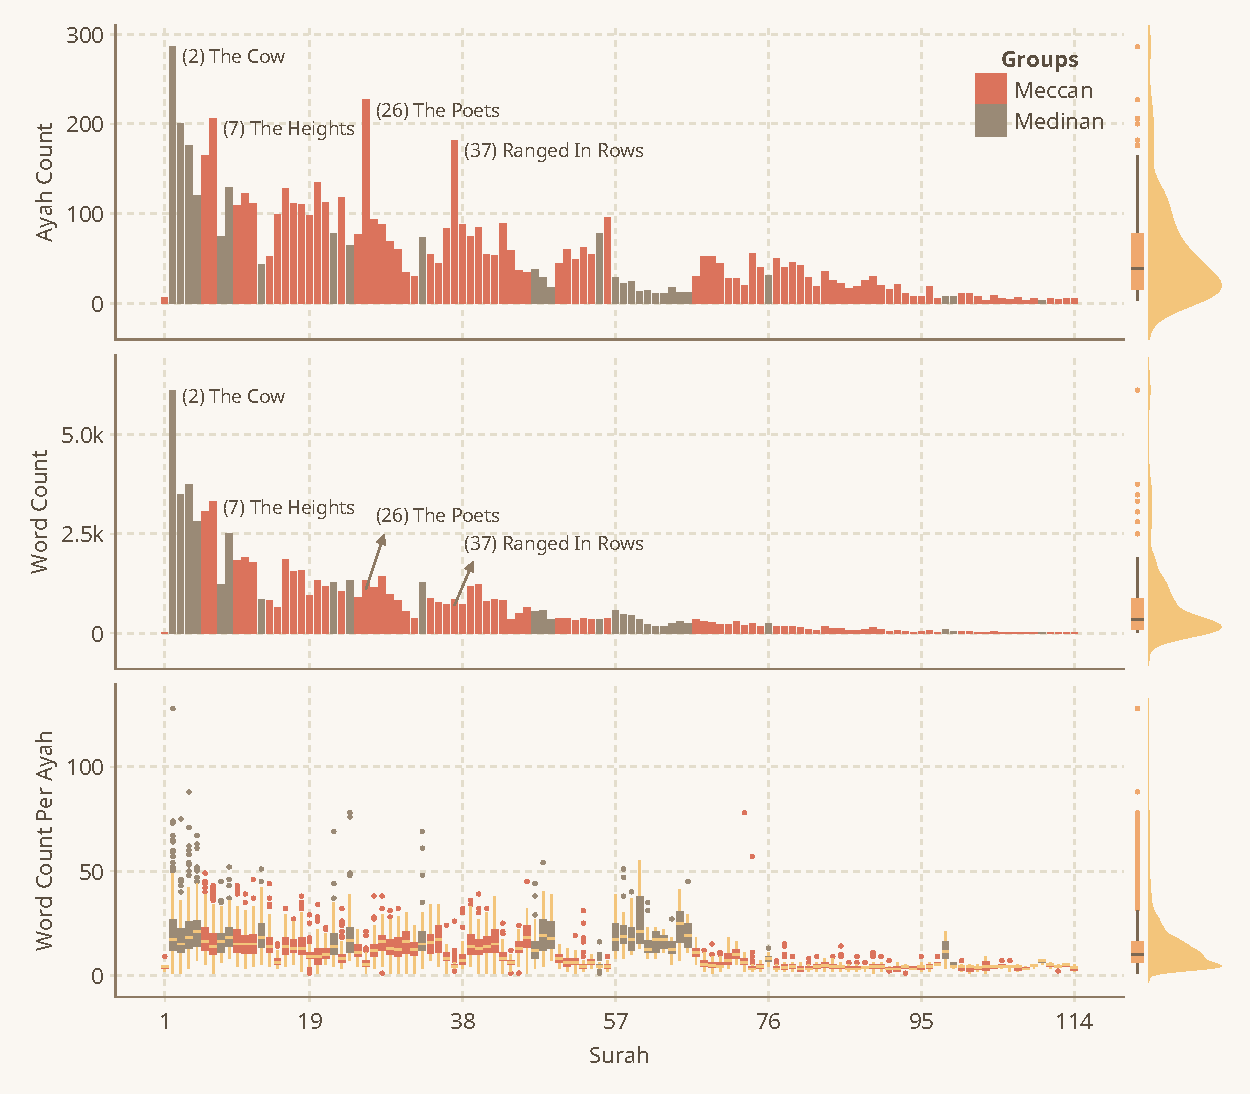
\includegraphics[height=0.7\textheight]{../img/plot1.pdf}
    \caption{Statistics of the words and \arb[trans]{'AyAt} \arb{'AyAt} (verses) of the Qur'\=an}
    \label{fig:ayah_word_count}
\end{figure}
\end{frame}

\begin{frame}[t, fragile]\justifying
\frametitle{Background and Motivation}
\begin{block}{The Qur'\=an}
\begin{itemize}\justifying    
\item Attempts at understanding the Qur'\=an by Qur'\=anic scholars were mostly done with the use of manual processes;\pause
\item However, with the advent of computers, some researchers have started using it to aid in their study. \pause
\item The first known to have used computers for studying the Qur'\=an was likely Rashad Khalifa in 1968\footnote{\url{https://www.masjidtucson.org/quran/miracle/a_profound_miracle_sura68nun133.html}}, where he studied the significance of the mysterious initials at the beginning of some \arb[trans]{sUwar} \arb{sUwar}.
\end{itemize}
\end{block}
\end{frame}

\begin{frame}[t, fragile]\justifying
\frametitle{Background and Motivation}
\begin{block}{The Qur'\=an}
\begin{itemize}\justifying        
\item Rashad uploaded the Qur'\=an into his computer by transliterating the Arabic letters and other Qur'\=anic orthographies into Roman letters and symbols that the computer can easily parse. This approach of using computers to find new insights is more common in the field of science, and it was new to the field of Qur'\=anic studies.\pause
\item Indeed, to proceed with the use of scientific computing, the Qur'\=an will be treated as the data that needs to be analyzed using a scientific process called Natural Language Processing (NLP), a branch of Machine Learning (ML) that aims to understand natural languages, such as Arabic.
\end{itemize}
\end{block}
\end{frame}

\begin{frame}[t, fragile]\justifying
\frametitle{Background and Motivation}
\begin{block}{The Qur'\=an}
\begin{itemize}\justifying        
\item To instruct the computer to do Statistical analyses or ML, one needs to use a \textit{software application} or a formal\footnote{"formal" because these languages were invented by man for particular purpose, in this case to communicate with computers} language called \textit{programming language}.\pause
\item The popular one for researchers in the field of sciences are Python \cite{van1995python}, R \cite{rprogramming}, and sometimes Julia \cite{Julia2017}. \pause
\item Therefore, if the data is the Qur'\=an, then there should be a way to interface with it using any of these programming languages. There are indeed some programming languages with libraries or packages for interfacing with the Qur'\=an, and this is true for Python, R, and \mbox{Julia}. 
\end{itemize}
\end{block}
\end{frame}

\begin{frame}[t, fragile]\justifying
\frametitle{Background and Motivation}
\begin{block}{The Qur'\=an}
\begin{itemize}\justifying    
\item For this study, the three programming languages will be used. \pause
\item The ruling is that Julia will be used for interfacing with the Qur'\=an texts since its library for it has more features \cite{asaad2021qurantree} compared to R and Python. \pause
\item The said Julia library is the QuranTree.jl\footnote{\url{https://alstat.github.io/QuranTree.jl/stable/}}. QuranTree.jl is based on Tanzil\footnote{\url{https://tanzil.net/download/}} for the Qur'\=anic Arabic texts, and \cite{dukes-habash-2010-morphological} for morphological annotation, which both libraries from R and Python do not have in terms of morphological annotations from \cite{dukes-habash-2010-morphological}. 
\end{itemize}
\end{block}
\end{frame}

\begin{frame}[t, fragile]\justifying
\frametitle{Background and Motivation}
\begin{block}{The Qur'\=an}
\begin{itemize}\justifying    
\item On the other hand, both R and Python will be used for libraries that are not available in Julia. In particular, R is known for niche statistical libraries since it was made for statistical computation, whereas Python is now popular for Deep Learning frameworks for complex modeling like TensorFlow\footnote{\url{https://www.tensorflow.org/}} (a library made by Google\footnote{\url{https://research.google/}}) and PyTorch\footnote{\url{https://pytorch.org/}} (a library made by Meta\footnote{\url{https://ai.meta.com/}}). 
\end{itemize}
\end{block}
\end{frame}


\begin{frame}[t, fragile]\justifying
\frametitle{Background and Motivation}
\begin{block}{The Qur'\=an}
\begin{itemize}\justifying    
\item Statistics is a branch of Science that aims to study features or characteristics of data generated from a random phenomenon. The findings of Statistical analyses can then be used to make decisions, conclusions or predictions of the general population of the data or general characteristics of the data. \pause
\item Machine Learning or ML, on the other hand, is a branch of Artificial Intelligence that heavily intersects with Statistics, albeit with distinct differences as well. Both Statistics and ML aims to characterize data by learning its features, but ML researchers have been aiming on complex models that are often inspired by simpler models from Statistics. Therefore, one can think of Statistics as one of the fundamentals of ML. 
\end{itemize}
\end{block}
\end{frame}

\begin{frame}[t, fragile]\justifying
\frametitle{Objectives}
The following are the general and specific objectives of this paper:
\begin{enumerate}
\item What are the structural characteristics of the Qur'an that can be extracted from its rich morphologies using statistical and large language models?\pause
\begin{enumerate}
    \item What are the statistics of the Qur'\=an's morphological features in terms of its parts of speech and selected entities like God's name and the prophets names mentioned?\pause
    
    \item How do the rhythmic signatures of the Qur'\=an of the verses looks like and what are statistical insights that can be extracted?\pause

    \item What are the rhythmic signatures of the \arb[trans]{'AyAt} \arb{'AyAt} of \arb[trans]{makkiyyaT} \arb{makkiyyaT} and \arb[trans]{madaniyyaT} \arb{madaniyyaT} \arb[trans]{sUwar} \arb{sUwar}?
\end{enumerate}
\end{enumerate}
\end{frame}

\subsection{Objectives}
\begin{frame}[t, fragile]\justifying
\frametitle{Objectives}
\begin{enumerate}
\setcounter{enumi}{1}
\item What other insights that can be extracted from the semantics of the Qur'an's texts using statistical and large language models?\pause
\begin{enumerate}
    \item How does the theory of \textit{concentrism} be formulated statistically, and what are the insights from the statistical and large language models on this? \pause
    
    \item How do the \arb[trans]{sUwar} \arb{sUwar} are organized in terms of the topics? What are the themes that can be extracted for each of the surahs?\pause
    
    \item How do these extracted themes compare to the summaries of Abdel\linebreak Haleem's English translation of the Qur'an?
\end{enumerate}\pause

\item How does these combinations of statistical, machine learning, and artificial intelligence with the Muslim's traditional literatures help in understanding the Qur'\=an, especially with the advent of Generative AI?
\end{enumerate}
\end{frame}

\subsection{Significance of the Study}
\begin{frame}[t, fragile]\justifying
\frametitle{Significance of the Study}
The significance of this study is that:
\begin{itemize}
    \item It brings forward new ways of extracting insights from the Qur'\=an by leveraging Computations, Statistics, Machine Learning, and AI, that is still in its early stage in the field of Qur'\=anic Studies. \pause
    \item This is especially true for Islamic Studies researcher, which the author hopes to benefit and get interested in Islamicate Digital Humanities, a new field which aims to take advantage of the scientific computations for studying Islamic texts, which the author hopes to have in any Islamic institute. \pause
    \item Further, since this paper combines the several fields (Islamic Studies, Statistics, and Machine Learning), the results will also contain mathematical theories that is hoped to advance the field of Statistics and Machine Learning as well.
\end{itemize}
\end{frame}

\begin{frame}[t, fragile]\justifying
\frametitle{Significance of the Study}
The significance of this study is that:
\begin{itemize}
\item With that said, the author would like to also emphasize the opportunities that scientific methodologies can bring to studying Islamic studies, especially for Muslim researchers who are in the field of science. \pause
\item Finally, this new perspective or process of studying the scripture not only aids the scholars of the Islamic Studies, Statistics, and Machine Learning, but may also contribute indirectly to community development and policy makers who use Qur'\=an as part of their decision making.
\end{itemize}
\end{frame}

\subsection{Scope of the Study}
\begin{frame}[t, fragile]\justifying
\frametitle{Scope of the Study}
The significance of this study is that:
\begin{itemize}
    \item The paper will cover all chapters of the Qur'\=an as much as possible, except maybe for cases like thematic modeling on very short \arb[trans]{sUwar} \arb{sUwar}, since topics on these \arb[trans]{sUwar} \arb{sUwar} may be obvious already or easier to see due to very short number of \arb[trans]{'ayaT} \arb{'ayaT}. 
    \item However, for cases where the analyses is not at the level of \arb[trans]{sUraT} \arb{sUraT}, but rather on the level of the Qur'\=an as a whole, then all of the \arb[trans]{sUwar} \arb{sUwar} will be used. 
\end{itemize}
\end{frame}

\subsection{Mathematical Sections}
\begin{frame}[t, fragile]\justifying
\frametitle{Mathematical Sections}
\begin{itemize}
    \item Like any humanities studies, Mathematics is mostly concern with understanding facts about objects that is being studied. 
    \item For Islamic studies, these objects can be physical like Qur'\=an and other Islamic texts, or metaphysical like understanding the purpose of life. \item For Mathematics, the objects can be explicit or abstract as well, but it does revolve heavily on numbers and logics, and like other domain it studies facts about these objects. 
    \item With that said, any object being studied in Mathematics are presented as Definitions, a formal way of defining terms or objects
\end{itemize}
\end{frame}

\begin{frame}[t, fragile]\justifying
    \frametitle{Mathematical Sections}
    \begin{block}{Mean}\label{defn:mean-1}
    Let $x_i, i\in\{1,\cdots,n\}$ where $n\in\mathbb{N}$, then the \textit{mean} of $x_i$s is defined as follows:
    \begin{equation}\label{eq:mean-formula-1}
        \bar{x} = \frac{1}{n}\sum_{i=1}^n x_i, \qquad\text{where}\;x_i \in\mathbb{R}.
    \end{equation}
    \end{block}
    \begin{itemize}
        \item Verified facts that are of significant findings are sectioned as Theorem in mathematics, whereas those that are proposed are called Proposition. 
        \item Other small results or facts supporting the Proposition are sectioned as Corollary.
    \end{itemize}
\end{frame}
    
\section{Review of Related Literatures}
\begin{frame}[t, fragile]\justifying
    \frametitle{Review of Related Literatures}
    \begin{itemize}
        \item The earliest paper on Qur'\=anic studies using computer was likely the work of Rashad Khalifa in 1968\footnote{\url{https://www.masjidtucson.org/quran/miracle/a_profound_miracle_sura68nun133.html}}, which led to one of his book entitled `The Computer Speaks: God's Message to the World' (\textit{see} \cite{rashad1981}).
        \item Rashad started at studying the mystery letters in the beginning of some \textit{s\=urahs} \arb{sUr} (for example Qur'\=an 2:1, 3:1, 7:1, etc.), it quickly went on to cover what he calls other \textit{mathematical miracles}, all of which are covered in \cite{rashad1981}.
        \item Rashad was able to do this by transliterating the Qur'\=an into Alpha-Numeric typesets for easy parsing of the computers back then.
    \end{itemize}
\end{frame}

\begin{frame}[t, fragile]\justifying
    \frametitle{Review of Related Literatures}
    \begin{itemize}
        \item Among the pioneers in computational applications for the Qur'\=an is the work of \cite{thabet2004}, who built a stemmer system for the Qur'\=an. \pause
        \item For example, in English language the root word for \textit{computational}, \textit{computer}, \textit{computation}, and \textit{computerize} is \textit{compute}. 
        \item According to \cite{thabet2004}, the rich morphology of the Qur'\=anic language or the Classical Arabic makes it even more difficult to do word stemming. 
    \end{itemize}
\end{frame}

\begin{frame}[t, fragile]\justifying
\frametitle{Review of Related Literatures}
\begin{itemize}
\item Moving on, \cite{thabet2005} builds on top of this stemming system, and used it for tokenization of the Qur'\=anic words, and building a statistical methodology for clustering or grouping the chapters of the Qur'\=an, in particular \cite{thabet2005} used a Agglomerative Hierarchical Clustering based on the Euclidean distance of the adjusted word frequency of a \arb[trans]{sUraT} \arb{sUraT}.
\item With the growing interests on studying the Qur'\=an from the lense of Data Analysis and Natural Language Processing, resulted into creating digital corpi of the Qur'\=an.
\item A series of work by Sharaf and Atwell led to the following publications: \cite{sharaf2009} studied knowledge representation of the Qur'\=an's verb valences using FrameNet frames, the output of which is a lexical database as a corpus of Qur'\=an's verbs. 
\end{itemize}
\end{frame}

\begin{frame}[t, fragile]\justifying
\frametitle{Review of Related Literatures}
\begin{itemize}
    \item Further, the work of \cite{sharaf2012} came up with corpus for the annotations of the Qur'\=anic pronouns, the authors named it as QurAna. 
    \item Building on this work, \cite{sharaf2012b} came up with a corpus for studying Qur'\=anic relatedness based on the commentary of Ibn Kathir \arb{ibn ka_tir}, the authors named this corpus as QurSim.
    \item Apart from Sharaf and Atwell, Dukes and Habash was also working on this, but specifically on the morphological annotations.
    \item For example, \cite{dukes-habash-2010-morphological}, which also led to other publications \cite{dukes2010online, dukes2013supervised, dukes2010dependency} related to this.
\end{itemize}
\end{frame}


\begin{frame}[t, fragile]\justifying
\frametitle{Review of Related Literatures}
\begin{itemize}
    \item With the establishment of a morphological annotated corpus for the Qur'\=an, the hoped was to have further analyses on the said scripture using statistical and machine learning methodologies. 
    \item As such, the work of \cite{dukes-habash-2011-one, dukes2015statistical} were among the first to do so, where they constructed a statistical parser through machine learning.
    \item This was then followed by \shortcite{siddiqui2013} who used the said corpus for topic modeling using Latent Dirichlet Allocation, the said study started with 114 \arb[trans]{sUwar} \arb{sUwar}, but after processing it went down to 24 \arb[trans]{sUwar} \arb{sUwar} after considering \arb[trans]{sUwar} \arb{sUwar} with 1000 or more words.dukes2010dependency} related to this.
\end{itemize}
\end{frame}


\begin{frame}[t, fragile]\justifying
    \frametitle{Review of Related Literatures}
    \begin{itemize}
        \item This was mainly due to the very sparse document term matrix for the Term Frequency - Inverse Document Frequency\footnote{\textit{See} Section \ref{sec:tf-idf}} (TF-IDF) embedding if considering all of the 114 \arb[trans]{sUwar} \arb{sUwar}.
        \item Aside from this, the rest have used the corpus by \cite{dukes-habash-2010-morphological} as part of benchmark for morphological analysis or for new lexicographic database, for example \cite{sabtan2017morphological, jarrar-hammouda-2024-qabas-open}.
    \end{itemize}
    \end{frame}
    With the establishment of a morphological annotated corpus for the Qur'\=an, the hoped was to have further analyses on the said scripture using statistical and machine learning methodologies. As such, the work of \cite{dukes-habash-2011-one, dukes2015statistical} were among the first to do so, where they constructed a statistical parser through machine learning. This was then followed by \cite{siddiqui2013} who used the said corpus for topic modeling using Latent Dirichlet Allocation, the said study started with 114 \arb[trans]{sUwar} \arb{sUwar}, but after processing it went down to 24 \arb[trans]{sUwar} \arb{sUwar} after considering \arb[trans]{sUwar} \arb{sUwar} with 1000 or more words. This was mainly due to the very sparse document term matrix for the Term Frequency - Inverse Document Frequency\footnote{\textit{See} Section \ref{sec:tf-idf}} (TF-IDF) embedding if considering all of the 114 \arb[trans]{sUwar} \arb{sUwar}. Aside from this, the rest have used the corpus by \cite{dukes-habash-2010-morphological} as part of benchmark for morphological analysis or for new lexicographic database, for example \cite{sabtan2017morphological, jarrar-hammouda-2024-qabas-open}.
\begin{frame}
\begin{center}
\begin{Huge}
\bfseries Thank you!
\end{Huge}
\end{center}
\end{frame}

\begin{frame}[allowframebreaks]
    \frametitle{References}
    % \bibliographystyle{apacite}
    % \bibliography{proposal_reference.bib}
    \printbibliography
\end{frame}
\end{document}